\documentclass{article}


\usepackage{arxiv}
\usepackage{subfigure}
\usepackage[utf8]{inputenc} % allow utf-8 input
\usepackage[T1]{fontenc}    % use 8-bit T1 fonts
\usepackage{hyperref}       % hyperlinks
\usepackage{url}            % simple URL typesetting
\usepackage{booktabs}       % professional-quality tables
\usepackage{amsfonts}       % blackboard math symbols
\usepackage{nicefrac}       % compact symbols for 1/2, etc.
\usepackage{microtype}      % microtypography
\usepackage{lipsum}
\usepackage{graphicx}
\usepackage{diagbox}
\usepackage{amsmath}
\usepackage{float}
\title{Parallel Acceleration for Gaussian Process}

\author{Han Liu}

\begin{document}
\maketitle

\begin{abstract}
Gaussian Process (GP) is a principled, practical and probabilistic approach in kernel methods, which gives advantages with respect to the interpretation of model predictions and provides a well-founded framework for learning and model selection. However, Gaussian Process can not be well applied to large datasets due to the scalability problems. In this paper, we firstly illustrate the details for the training and testing of GP, and implement it with Tensorflow and Adam Optimizer. Then we combine several algorithms to accelerate the GP and try to compare it with the unaccelerated GP in time cost. The experiment shows that accelerated GP is nearly ten times faster than unaccelerated GP. In the future, a more intergral blackbox interface targeted at multi-output GP could be invertigated to further improve the scalability of GP.
\end{abstract}


% keywords can be removed
\keywords{Gaussian Process \and Parallel Computing \and Conjugate Gradient}


\section{Introduction}
In machine learning, kernel methods are  popular deep learning techniques which are used for pattern recognition, linear regression and correction analysis. Among kernel methods, Gaussian processes (GP) provide a principled, practical, probabilistic approach to learning in kernel machines \cite{1}. This gives advantages with respect to the interpretation of model predictions and provides a well-founded framework for learning and model selection. \\
\indent Theoretical and practical innovations of GP over the recent decades have developed rapidly. For instance, J. P. Cunningham et al. have proposed a fast Gaussian Process Methods for point process intensity estimation which can eliminate the memory burden and reduce the solve time by orders of magnitude. In 2003, A. Girard et al. use the non-parametric Gaussian process to solve the problem of multi-step ahead prediction in time series \cite{2}. Also, A. G. Wilson proposed a fast automatic pattern discovery and extrapolation with Gaussian processes by new covariance kernels \cite{3}. \\
\indent However, Gaussian Process has some fatal flaws: when the dataset become large, the traing process will become extremely slow. That is, the GP inference can not effectively applied to big data, which is the mainstream recently. Therefore, some approaches must be implemented to improve the scability of Gaussian Process. \\
The most common inference engine for GP is Cholesky decomposition, which is used for get the inversion and determinant of the kernel matrix. However, the Cholesky decomposition is fully serial, which is computional expensive. There are several approaches to solve this problem. For example, Conjugate Gradient (CG) algorithm can be used to get the matrix inverse with more ease \cite{4}, Lanczos tridiagonalization (LT) algorithm can be used to get the determinant of a positive definite matrix \cite{5}, Pivoted Cholesky decomposition (PCD) is an efficient algorithm for computing a low-rank decomposition of the kernel matrix \cite{6} and stochastic trace estimation (STE) algorithm can be used to estimate the trace of a matrix \cite{7}, etc. In 2018, J. R. Gardner et al. have proposed  a highly efficient framework for Gaussian Process inference, which combines CG algorithm, LT algorithm and STE algorithm as a whole. However, due to the numerical stability issues of LT algorithm, the estimation of log determinant is quite inaccurate, therefore, we must tackle this problem to obtain a better estimation of hyperparameters. In 2017, C. Boutsidis proposed a novel randomized algorithm for approximating the log determinant of a symmetric potive definite matrix, which is highly accurate and can be easily parallelled. In this paper, we try to modify this algorithm to make it adaptable for the training of GP.\\
This paper is organized as following: in the first part, we try to illustrate the details for the training and testing of GP, and implement it with Tensorflow and Adam Optimizer. In the second part, we combine several algorithms to accelerate the GP and try to compare it with the original version in both accuracy and cost time.

\section{Implementation of Gaussian Process}
In this section, we try to illustrate all the mathematical details of GP with according provement. Specifically, we will show how to learn the hyperparameters in the kernel function during the training process, how to predict the output given specific input during the testing process. Also, we will show the details in implementing GP with Tensorflow and Adam Optimizer. 
\subsection{Preliminary}
Broadly speaking, GP is a function that maps a set of random variables to another set of random variables, and there are two quantatives to specify the function: mean and covariance matrix. Generally, the mean is set to 0 and the covariance matrix is defined by kernel function. 
\subsubsection{Kernel Function}
The kernel function must be symmetric and positive definite and is used to determine the covariance matrix of different variables. It has many different types:
\begin{itemize}
	\item Squared Exponential Kernel (RBF): $k(x,x^{'})=s^2exp(\frac{-(x-x^{'})^2}{2\gamma^2})$
	\item Laplace Kernel: $k(x,x^{'})=s^2exp(\frac{-|x-x^{'}|}{\gamma})$
	\item Indicator Kernel: $k(x,x^{'})=I(x=x^{'})$
	\item Linear Kernel: $k(x,x^{'})=x^{T}x^{'}$
\end{itemize}
It is worth mentioning that more complicated kernels can be constructed by adding these classic kernel functions together. There is still another problem that need to be answered. When there are multiple input features among one single sample, these kernel could not work, as all the input must be scalars. Therefore, we must make some modifications to the original scalar form. Take the most common kernel RBF for example, we use the norm operation to denote it:
\begin{equation}
k(x,x^{'})=s^2exp(-\frac{||x-x^{'}||^2}{2l^2})
\end{equation}
In this case, it can be well suited in the multi-variable problems.
 \subsubsection{Training Process}
Suppose $x_i$ is the input of the training samples, $y_i$ is the output of the training samples, $\hat{f}$ is the estimation function of GP, $\sigma_i$ is the standard deviation and $\sum$ denote the covariance matrix obtained by kernel function. We suppose that the output values from the training samples are about $\hat{f}$  independent and obey Gaussian distribution, therefore, we can write the possibility as following:
\begin{equation}
p({y}|\hat{f})=\prod_{i=1}^{n}\frac{1}{\sqrt{2\pi \sigma_i^2}}exp(-\frac{(y_i-\hat{f}(x_i))^2}{2\sigma_i^2})
\end{equation}
 In the training process, the goal is to maximize the posterior probability, which is:
 \begin{equation}
 p(y|\sum)=\int p(y|f)p(f|\sum)df
 \end{equation}
 By using the property of GP, we can get:
 \begin{equation}
 p({y|\sum})\sim N(0,\sum+\sigma^2I_{00})
 \end{equation}
 Where $\sigma^2I_{00}$ is the variance matrix of $y_i$. Let $K$ denotes $\sum+\sigma^2I_{00}$, by expanding it into Gaussian expression: 
 \begin{equation}\label{eq1}
 logp({y|K})=-\frac{1}{2}log((2\pi)^k|K|)-\frac{1}{2}y^T{K}^{-1}y
 \end{equation}
 
 We can set the opposite of it as the loss function, as the minimization of the loss can lead to the maximization of the posterior probability. As for the training of GP, we always need to get the gradients of the loss function with respect to the hyperparameters. Suppose we use RBF kernel, and let $\theta$ represent $s^2$ and $\gamma$, as the derivation of gradients are quite similar at the beginning. As for a symmetric positive matrix, we have:
 \begin{equation}
 log|K|=tr(log(K))
 \end{equation}
 Take the gradient with respect to $\theta$:
 \begin{equation}
 \frac{\partial}{\partial \theta}(log|K|)=tr(K^{-1}\frac{\partial K}{\partial \theta})
 \end{equation}
 For the inverse of the gradient:
 \begin{equation}
 \frac{\partial K^{-1}}{\partial \theta}=-K^{-1}\frac{\partial K}{\partial \theta}K^{-1}
 \end{equation}
 Therefore, the gradient of the loss function is:
 \begin{equation}\label{eq2}
 \frac{\partial logp({y|K})}{\partial \theta}=-\frac{1}{2}[tr(K^{-1}\frac{\partial K}{\partial \theta})-y^TK^{-1}\frac{\partial K}{\partial \theta}K^{-1}y]
 \end{equation}
 
 \subsubsection{Testing Process}
 The principle of testing is quite intuitive. By the property of the joint Gaussian distribution, we can get the posterior probability:
 \begin{equation}
 p(\hat{y}|{y})\sim N(\sum_{10}K^{-1}y,\sum_{11}-\sum_{10}K^{-1}\sum_{01})
 \end{equation}
 Where $\sum_{10}$ is the covariance matrix between test samples and train samples and $\sum_{11}$ is the covariance matrix between the test samples. After getting mean and covariance matrix, it is easy to write the expression:
 \begin{equation}
 f(x_1,x_2,...,x_k)=\frac{1}{\sqrt{(2\pi)^k|\sum|}} exp(-\frac{1}{2}(x-u)^T\sum^{-1}(x-u)
 \end{equation}
 
 
\subsection{Methodology}
In this section, we will illustrate the theoretical basis for experiment section. Specifically, we firstly explain the design details for Tensorflow, then for Adam Optimizer.  
\subsubsection{Implementing with Tensorflow}
Tensorflow provides a quite efficient and integrated framework for learning hyperparameters. In this case, we only need to write the cost function with no need to write the explicit expression of the gradients. That is, we only need to write Equation \ref{eq1} with specifying $\gamma$ and $s$ as varaibles. We choose the learning rate as 0.001.

\subsubsection{Implementing with Adam Optimizer}
Adam Optimization is an adaptive learning rate optimization algorithm that’s been designed specifically for training deep neural networks \cite{8}. The most notable feature is that Adam uses estimations of first and second moments of gradient to adapt the learning rate during the training process. To estimate these moments, Adam utilizes exponentially moving averages, computed on the gradient evaluated on a current mini-batch:

\begin{equation}
\begin{split}
m_t=\beta_1m_{t-1}+(1-\beta_1)g_t    \\
v_t=\beta_2v_{t-1}+(1-\beta_2)g_t^2
\end{split}
\end{equation}
It our approach, I choose $\beta_1=0.9$ and $\beta_2=0.999$, the vectors of moving averages are initialized with zeros at the first iteration. Next, we need to correct the estimator to be unbiased as following:
\begin{equation} \label{eqn2}
\begin{split}
\hat{m_t}=\frac{m_t}{1-\beta_1^t}    \\
\hat{v_t}=\frac{v_t}{1-\beta_2^t}
\end{split}
\end{equation}
The last thing to do is to use those moving averages to scale learning rate individually for each parameter:
\begin{equation}
w_t=w_{t-1}-\eta\frac{\hat{m_t}}{\sqrt{\hat{v_t}+\epsilon}}
\end{equation}

\subsection{Experiment}
\subsubsection{Results of Tensorflow}
Firstly, we implement GP with tensorflow and predict the results in $f(x)=xsinx$. A comparison between the SK-learn and Tensorlfow is as following:
\begin{figure}[H]
	\centering
	\subfigure[Tensorflow]{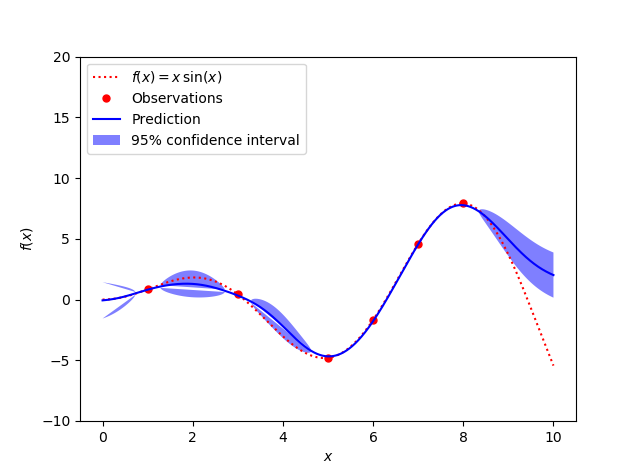
\includegraphics[width=2.7in]{my_test}}
	\subfigure[Sk-learn]{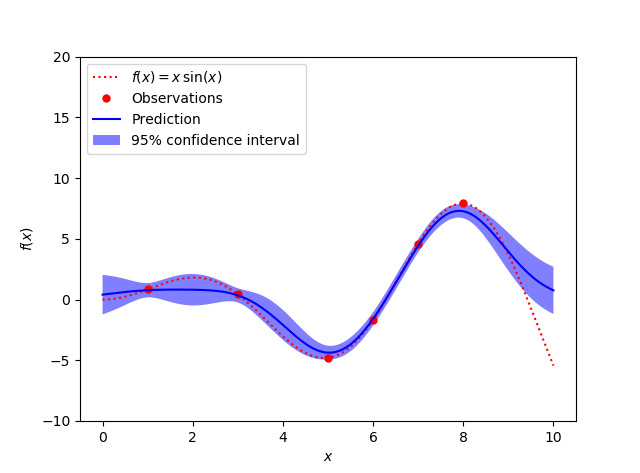
\includegraphics[width=2.7in]{skl}}
	\caption{Comparison of Two Implementations}
	\label{fig1}
\end{figure}
Obviously, we achieve a better accuracy compared to Sk-learn since the 95\% confidence interval is more tight. However, they all suffer from the problem of terrible predicting in the latter part of the function. We will discuss it in more details in the following section.
\subsubsection{Results of Adam Optimizer}
As for Adam optimizer, we still test it on function $f(x)=xsinx$. A comparison of the loss between Adam and Tensorflow is as following:
\begin{figure}[H]
	\centering
	\subfigure[Adam]{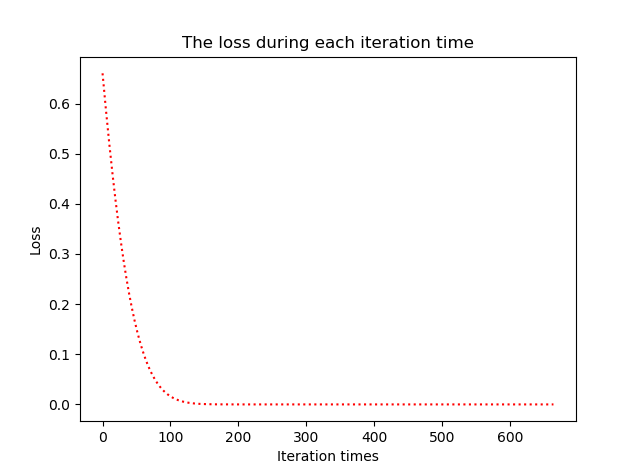
\includegraphics[width=2.7in]{adam_loss}}
	\subfigure[Tensorflow]{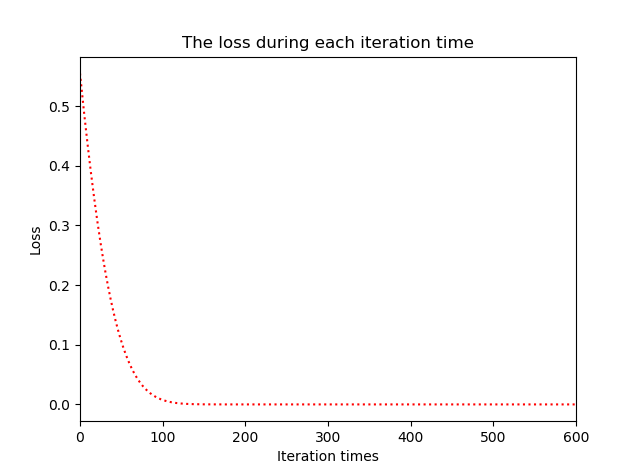
\includegraphics[width=2.7in]{tf_loss}}
	\caption{Comparison of Two Implementations}
	\label{fig2}
\end{figure}
From the above figures, it is clear to see they have linearly the same speed of convergence. But at the begining, Tensorflow methods have a smaller error, this is due to a better initialization of parameters embeded in Tensorflow. 
\subsubsection{Comparison with Other Methods}
 To show the competiveness of GP, we compare GP with many common regression methods. Specifially, we choose Forest Fires Dataset from UCI Machine Learning Repository \cite{9}. We divide training set and testing set with a ratio of 7:3. Then we test Linear Regression, Ridge Regression, Lasso Regression, Bayesian Ridge Regression, Theil-Sen Regression and Gaussian Process on the dataset, the error is calculated as following:
 \begin{equation}
 E=1/(1000N)\sum_{i=1}^{N}(y_i-\hat{y_i})^2
 \end{equation}
 Where I divide 1000 to make the comparison more notable. The results are as following:
  \begin{figure}[H]
 	\begin{center}
 		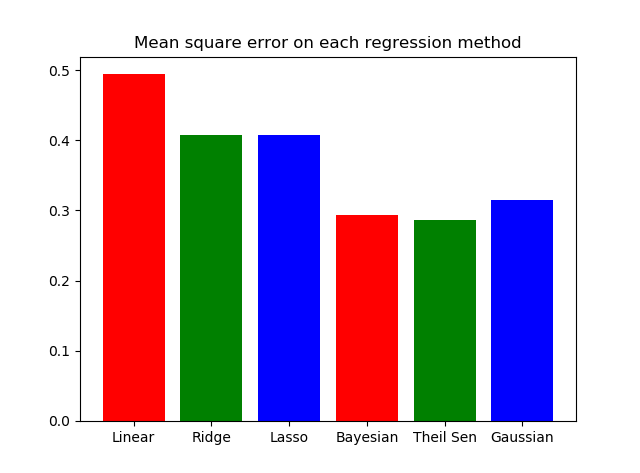
\includegraphics[width=0.5\textwidth]{non_interpolation_comparison}
 	\end{center}
 	\caption{Results of Several Regression Methods }
 	\label{fig3}
 \end{figure}
 From the above comparison, we can see that Bayesian, Thei Sen and Gaussian all achieve a similar accuracy, there is no obvious advantages of GP over other Regression methods. However, the performance of GP can be improved significantly if we use interpolation. We uniformly sample the training set with the same percentage 0.7, the results are as following:
   \begin{figure}[H]
 	\begin{center}
 		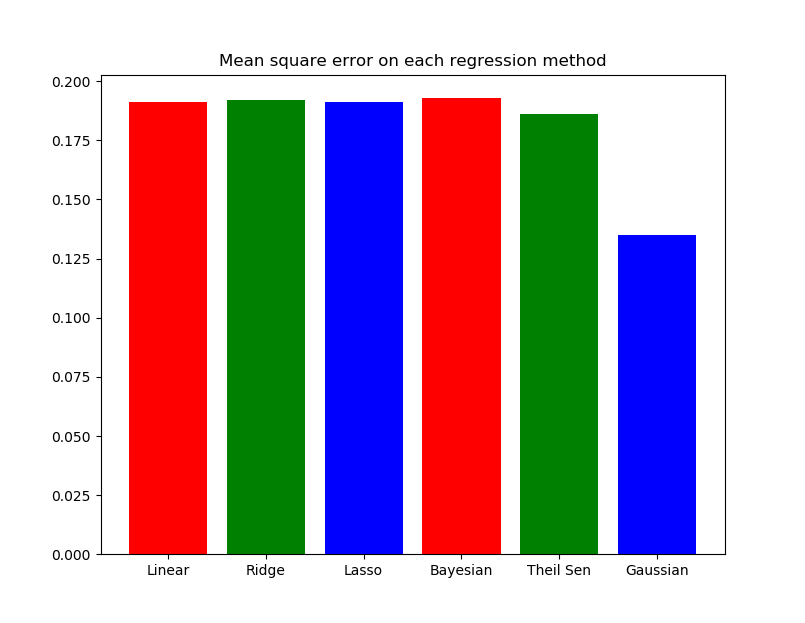
\includegraphics[width=0.5\textwidth]{Interpolation_comparison}
 	\end{center}
 	\caption{Results of Several Regression Methods Using Interpolation}
 	\label{fig4}
 \end{figure}
It is trival that Gaussian Process achieve a much better accuracy over other regression methods.

\section{Parallel Acceleration of Gaussian Process}
In this section, we illustrate several algorithms to accelerate Gaussian Process. Specifically, we will firstly use Modified Conjugate Gradient Algorithm to get the inverse of the matrix, then we will use Pivoted Cholesky Decomposition to precondition CG algorithm. Next, we will use Stochastic Trace Estimation to get the trace of kernel matrix. Also, we will show the flaws of Lanczos Tridiagonalization, and try to replace it with a new method: randomized algorithm. Lastly, we will compare the cost time between the accelerated version and original version. 
\subsection{Methodology}
In the process of training and predicting GP, we need to obtain the explicit expression of loss function given in Equation \ref{eq1} and gradients given in Equation \ref{eq2}. There are three quantities in these expressions that dominate its time complexity: $K^{-1}y$, $log|K|$, $tr(K^{-1}\frac{\partial K}{\partial \theta_j})$. Before that, Cholesky decomposition is used to get all these three quantities. However, Cholesky decomposition is highly serial, which is very computational expensive, thus we need some computional algorithm that can be parallelled to improve the scability of GP over large datasets.\\
\subsubsection{Modified Conjugate Gradient}
Conjugate Gradient is a common method used for calculating the product of the matrix inverse and a vector. Its algorithm flow chart is as following \cite{10}:

   \begin{figure}[H]
	\begin{center}
		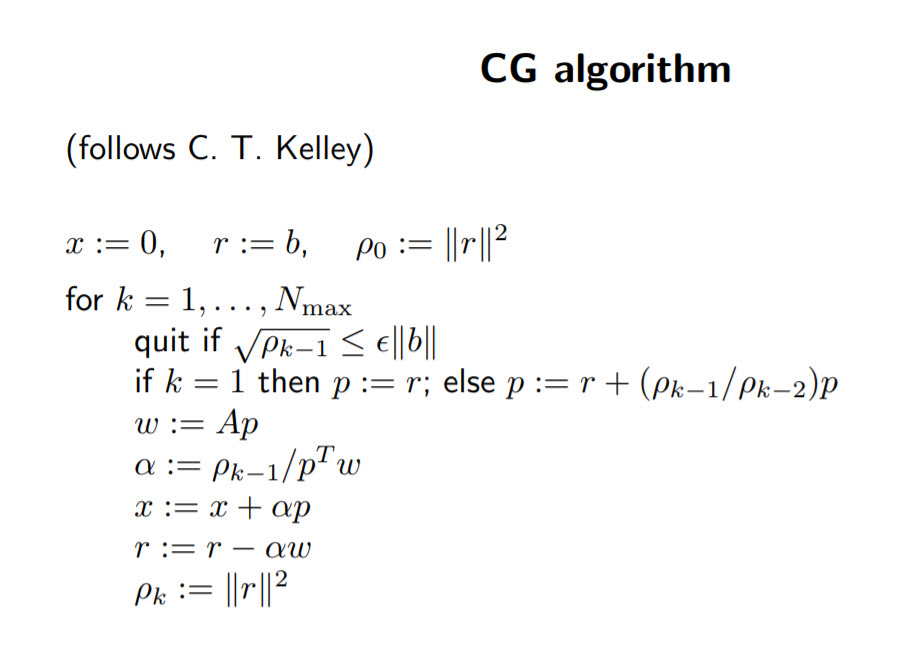
\includegraphics[width=0.6\textwidth]{CG}
	\end{center}
	\caption{Conjugate Gradient Algorithm}
	\label{fig5}
\end{figure}
It is quite fast to get the inverse product compared to normal calculation, we will demonstrate it in experiment section.\\
Modified Conjugate Gradient (mCG) is a parallel form of CG algorithm. Specifically, we will use mCG to calculate:
\begin{equation}\label{equ1}
[u_0 \quad u_1 \quad ... \quad u_t]=K^{-1}[y \quad z_1 \quad ... \quad z_t]
\end{equation} 
Where $z_1 \quad ... \quad z_t$ are uniformly distributed random variables, these quantities are quite useful when determining  $tr(K^{-1}\frac{\partial K}{\partial \theta_j})$, we will illustate it in later part.
\subsubsection{Pivoted Cholesky Decomposition}
Pivoted Cholesky Decomposition (PCD) is mainly used for preconditioning \cite{11}. The basic idea of preconditioning is to introduce a matrix $P$ to solve the linear system:
\begin{equation}
P^{-1}\hat{K}u=P^{-1}y
\end{equation}
The preconditioning will guarantee to have the same solution with the original linear system, and the system’s convergence is depend on the conditioning of $P^{-1}\hat{K}$ rather than $\hat{K}$. Furthermore, if $P^{-1}\hat{K}\approx I$, the system will converge fastly, thus Pivoted Cholesky Decomposition is very useful to precondition the CG algorithm. \\
As for PCD algorithm, the idea is to produce a low rank approximation of a positive definite matrix:
\begin{equation}
K_{xx}=L_kL_k^T
\end{equation}
Where $L_k$ is the triangular matrix. The difference between traditional Cholesky Decomposition and PCD is that PCD always swap the maximum diagonal element to the top left corner of the matrix. The pseudo-code of PCD is as following:
  \begin{figure}[H]
	\begin{center}
		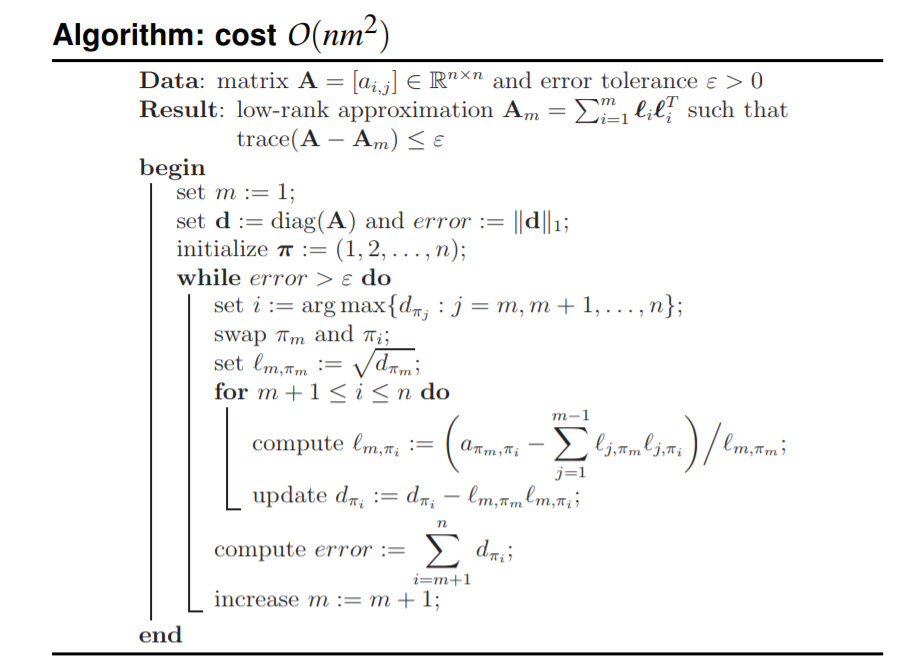
\includegraphics[width=0.6\textwidth]{PCD}
	\end{center}
	\caption{Pivoted Cholesky Decomposition}
	\label{fig6}
\end{figure}

\subsubsection{Stochastic Trace Estimation}
Stochastic Trace Estimation (STE) is an efficient algorithm to determine the trace of a matrix \cite{12}. The idea is to introduce a set of uniformly distributed independent random variables with the equal probability on -1 and 1 to estimate the trace. That is:
\begin{equation}
Tr(K)=E(z_i^TKz_i)
\end{equation}
Where $K$ is any matrix, $z_i$ is random variable. We can use the numerical mean to estimate the exact mean:
\begin{equation}
E(z_i^TKz_i)=\frac{1}{N}\sum_{i=1}^{N}z_i^TKz_i
\end{equation}
The arithmetic mean will converge to the exact mean with the increasing of $N$. This algorithm is useful to determine $tr(K^{-1}\frac{\partial K}{\partial \theta_j})$:
\begin{equation} \label{21}
tr(K^{-1}\frac{\partial K}{\partial \theta_j})=E[z_i^TK^{-1}\frac{\partial K}{\partial \theta_j}z_i]
\end{equation}
We can use CG algorithm to calculate Equation \ref{equ1} to get $u_i=K^{-1}z_i$, then $u_i^T=z_i^TK^{-1}$. Therefore, we just need to multiply the gradient part to get Equation \ref{21}.
\subsubsection{Lanczos Tridiagonalization}
The Lanczos Tridiagonalization (LT) \cite{13} is an iterative MVM-based procedure to obtain a tridiagonalization of a symmetric matrix A. A tridiagonalization is a decomposition $A=QTQ^T$ with $Q\in R^{n\times n}$ orthonormal and $T\in R^{n\times n}$ tridiagonal. It is shown that n iterations of this algorithm produces an exact tridiagonalization $A=QTQ^T$, $p$ iterations yield a low-rank approximate tridiagonalization $A\approx \tilde{Q}\tilde{T}\tilde{Q}^T$, where $\tilde{Q} \in R^{n\times p}$ and $\tilde{T}\in R^{p\times p}$. \\
LT algorithm is useful to calculate $log|K|$. As we can produce an exact tridiagonalization $K=QTQ^T$, then by the property of determinant:
\begin{equation}
det(K)=det(Q)det(T)det(Q^T)
\end{equation}
Also, since $Q$ is orthonormal, we have $det(Q)=det(Q^T)=\pm 1$, so we can get: $det(K)=det(T)$.\\
However, this algorithm could suffer from the loss of orthogonality during the iteration time due to the rounding errors. This could has several impacts on the accuracy of the above estimation, as the orthonormal condition no longer holds. In the experiment section, I will illustrate it in more details.
\subsubsection{Randomized Algorithm}
Randomized Algorithm is another novel algorithm for approximating the logarithm of the determinant of a symmetric positive definite matrix \cite{14}. There are three steps for the implementation of Randomized Algorithm:
\begin{enumerate}
	\item Compute some $\alpha$ with $\lambda_1(A)<\alpha$
	\item Compute $C=I_n-A/\alpha$
	\item Compute the trace of all the powers of $C$ 
\end{enumerate}
Where $A$ is the matrix that we want to get the determinant, $I_n$ is a $n\times n$ identity matrix, $\lambda_1(A)$ is the maximum eigen value of $A$. The formula for calculating logdet of $A$ is:
\begin{equation}
log|A|=nlog(\alpha)-\sum_{k=1}^{m}(\frac{1}{p}\sum_{i=1}^{p}g_i^TC^kg_i)/k
\end{equation}
We can use Power Method to calculate the largest eigen value $\lambda_1(A)$. $m$ denote the order of the expansion, with the increase of $m$, the algorithm will be more accurate but also takes more running time, a detailed investigation of the impact of $m$ is given in experiment section.




\subsection{Experiment}
In this section, we will evaluate the effectiveness of the above algorithms by experiment. Specifically, in the first part, we will show the faster speed of CG algorithm compared to traditional inverse calculation; in the second part, we will show the convergence of STE algorithm; in the third part, we will show the flaws of LT algorithm with possible reasons; in the fourth part, we will show the accuracy and the impacts of $m$ on the Randomized Algorithm; lastly, we will show the overall performance of Parallel Acceleration over original version.
\subsubsection{Results of Modified Conjugate Gradient}
We test the time cost of $K^{-1}y$ on a set of order-n matrix $K$ by exact inverse and CG algorithm, the results are as following:
  \begin{figure}[H]
	\begin{center}
		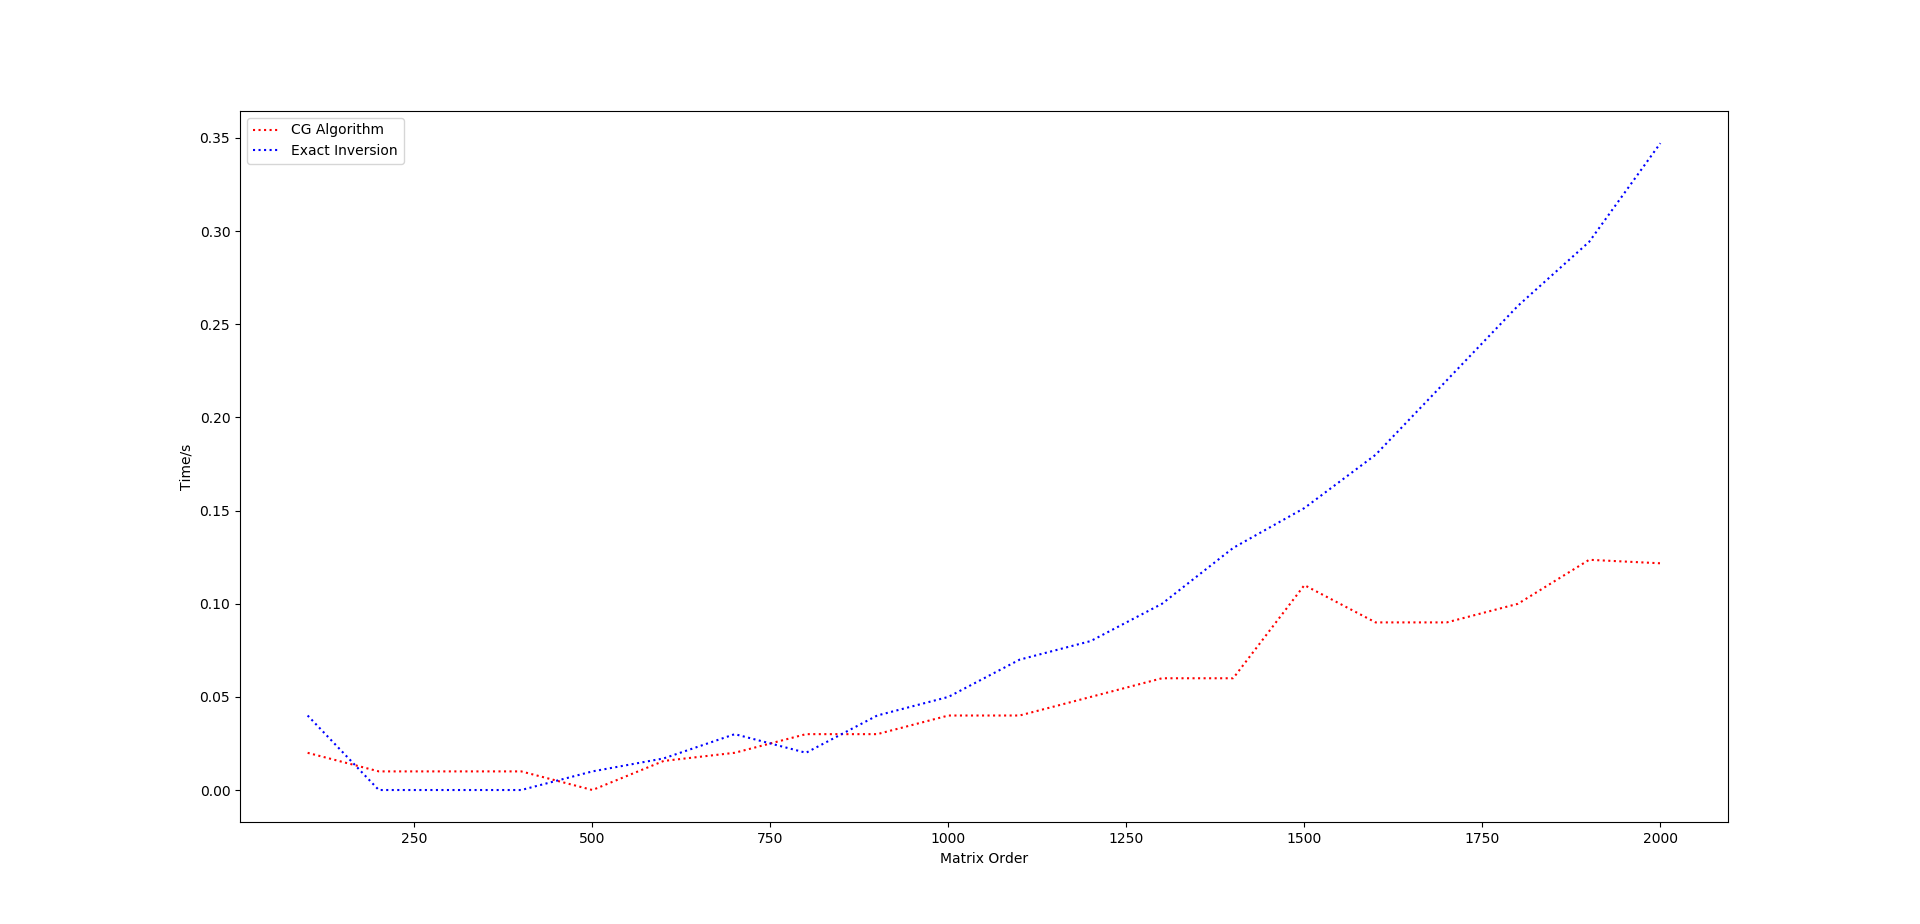
\includegraphics[width=0.75\textwidth]{CG_time}
	\end{center}
	\caption{Time Cost of Inverse Computation by CG and Exact Inverse}
	\label{fig7}
\end{figure}
From the above figure, it is clear to see that when the order of the matrix is small (below 1000), the two algorithms have nearly the same performance. However, when the order is large, CG spends much less time than exact inverse, and the larger $m$ is, the more time saved.

\subsubsection{Results of Stochastic Trace Estimation}
To show the convergence of Stochastic Trace Estimation, we test this algorithm on a randomly-generated $15\times15$ matrix, the results are as following:
  \begin{figure}[H]
	\begin{center}
		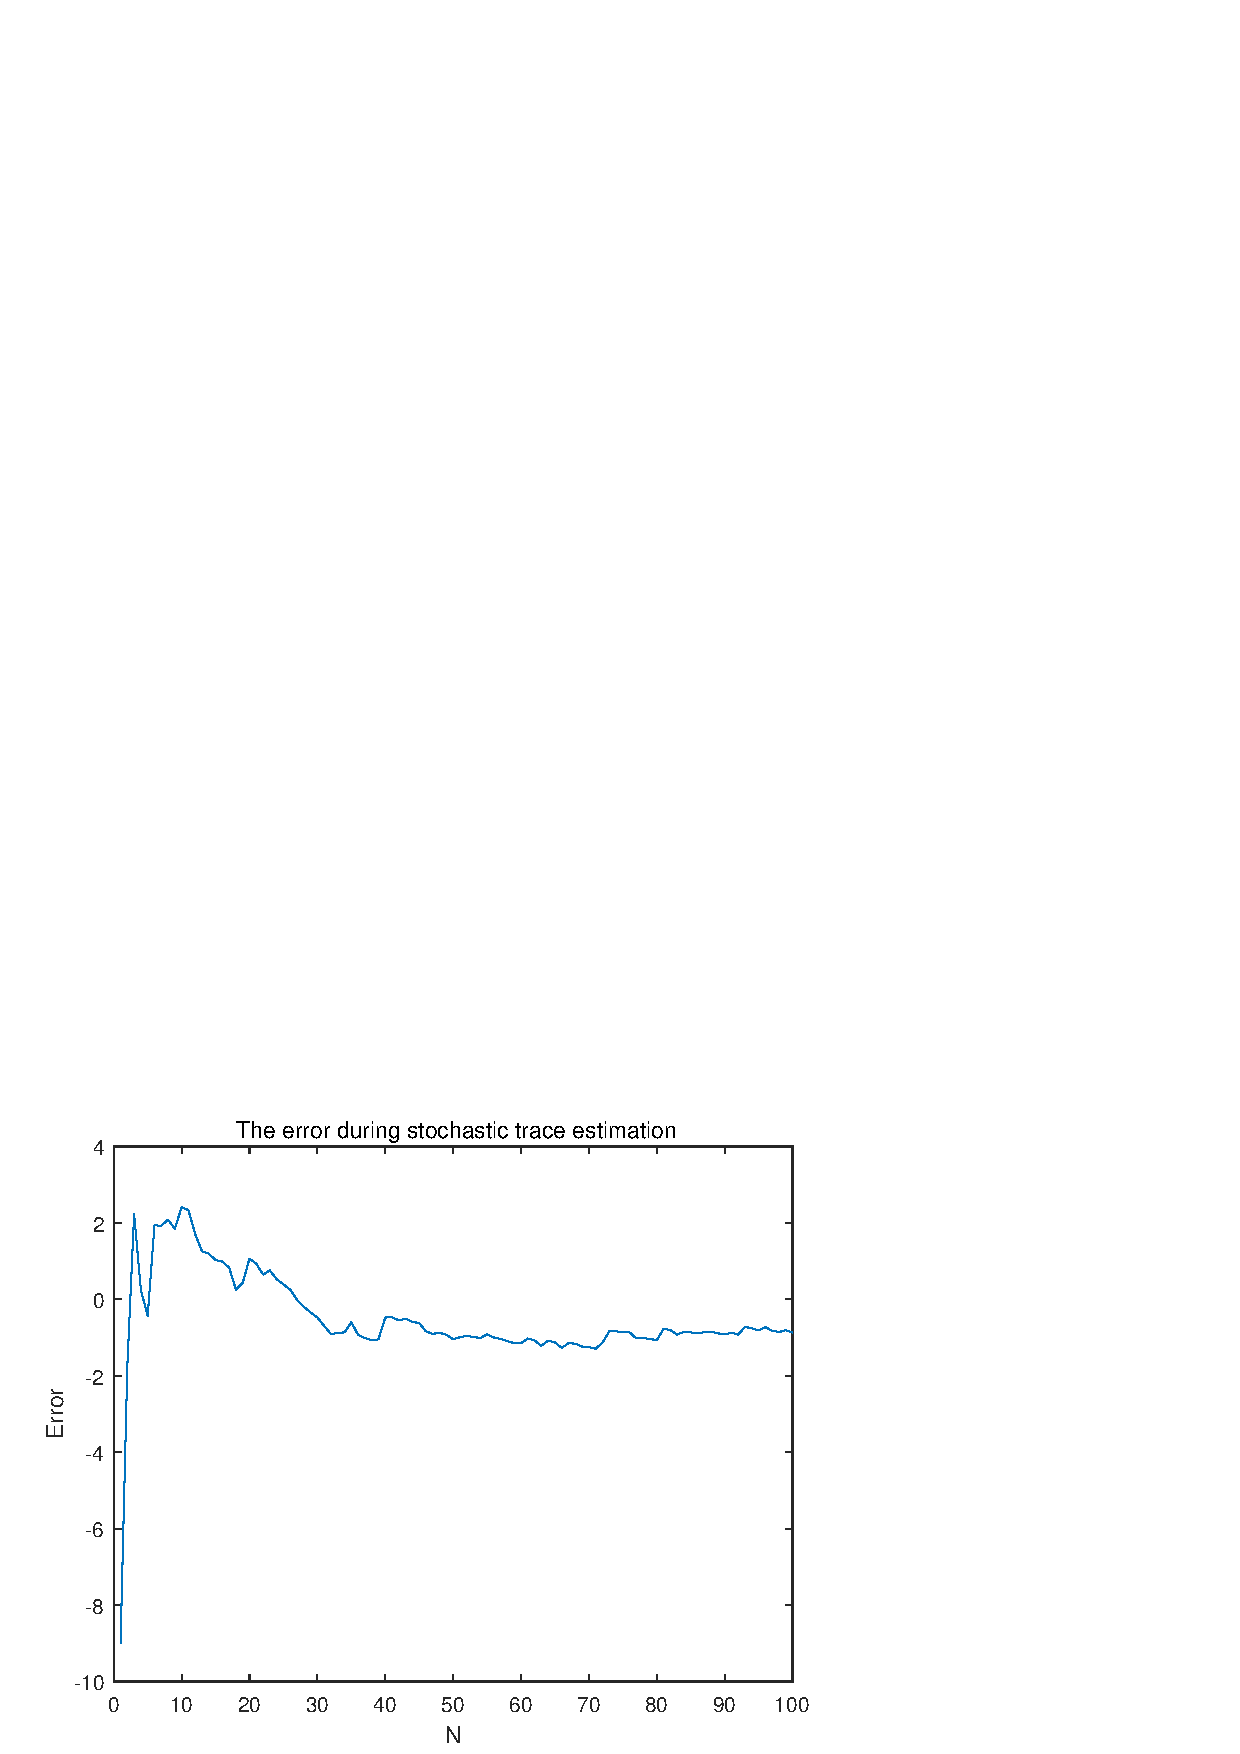
\includegraphics[width=0.7\textwidth]{error}
	\end{center}
	\caption{The Error of Stochastic Trace Estimation During Each Iteration}
	\label{fig8}
\end{figure}
From the above figure, when $N$ approach 20, the error reaches nearly $0$, this result also holds for large matrix.


\subsubsection{Results of Lanczos Tridiagonalization}
Due to the finite precison of machines, the Lanczos Tridiagonalization will lose orthogonality very quickly. To demonstrate this, we choose a randomly-generated $8\times 8$ matrix, which will produce $K=QTQ^T$ according to the algorithm. We multiply $Q$ with $Q^T$, the results are as following: 
\begin{table}[htbp]
	\centering
	\caption{Multiplication Results of $Q$ and $Q^T$}
	\begin{tabular}{rrrrrrrrr}
		\toprule
	    & 1     & 2     & 3     & 4     & 5     & 6     & 7     & 8 \\
		\midrule
		1     & 1     & 2.5E-16 & 2.95E-16 & -2.2E-14 & 4.11E-12 & -7.8E-12 & 0.467695 & -0.36042 \\
		2     & 2.5E-16 & 1     & -3.6E-16 & 5.77E-15 & -1.9E-12 & 1.31E-11 & -0.81702 & -0.32851 \\
		3     & 2.95E-16 & -3.6E-16 & 1     & 1.5E-14 & -1.6E-12 & -7.3E-12 & 0.331487 & -0.4423 \\
		4     & -2.2E-14 & 5.77E-15 & 1.5E-14 & 1     & 8.94E-15 & -1.7E-13 & -0.06215 & -0.75269 \\
		5     & 4.11E-12 & -1.9E-12 & -1.6E-12 & 8.94E-15 & 1     & -8.8E-16 & -0.00022 & -0.00405 \\
		6     & -7.8E-12 & 1.31E-11 & -7.3E-12 & -1.7E-13 & -8.8E-16 & 1     & 4.13E-05 & -0.00013 \\
		7     & 0.467695 & -0.81702 & 0.331487 & -0.06215 & -0.00022 & 4.13E-05 & 1     & -2.1E-15 \\
		8     & -0.36042 & -0.32851 & -0.4423 & -0.75269 & -0.00405 & -0.00013 & -2.1E-15 & 1 \\
		\bottomrule
	\end{tabular}%
	\label{tab1}%
\end{table}%
From Table \ref{tab1}, it is clear to see the first six columns of this matrix are orthogonal to each other, but the last two columns are not. This phenomenon is called the loss of orthogonality. This will cause a severe influence on the accuracy of $log|K|$, as the conditon of orthogonality no longer holds.\\
There are many measures to tackle this problem. For example, H. D. Simon proposed a Lanczos algorithm with partial reorthogonalization \cite{15} to maintain orthogonality among the Lanczos vectors during the iterations. In our case, we use a new method: randomized algorithm to calculate the log determinant. 

\subsubsection{Results of Randomized Algorithm}
As for Randomized Algorithm, we firstly evaluate the effect of $m$. We test this algorithm on $100\times 100$ matrix with a set of $m$, and we use relative error as the benchmark.
  \begin{figure}[H]
	\begin{center}
		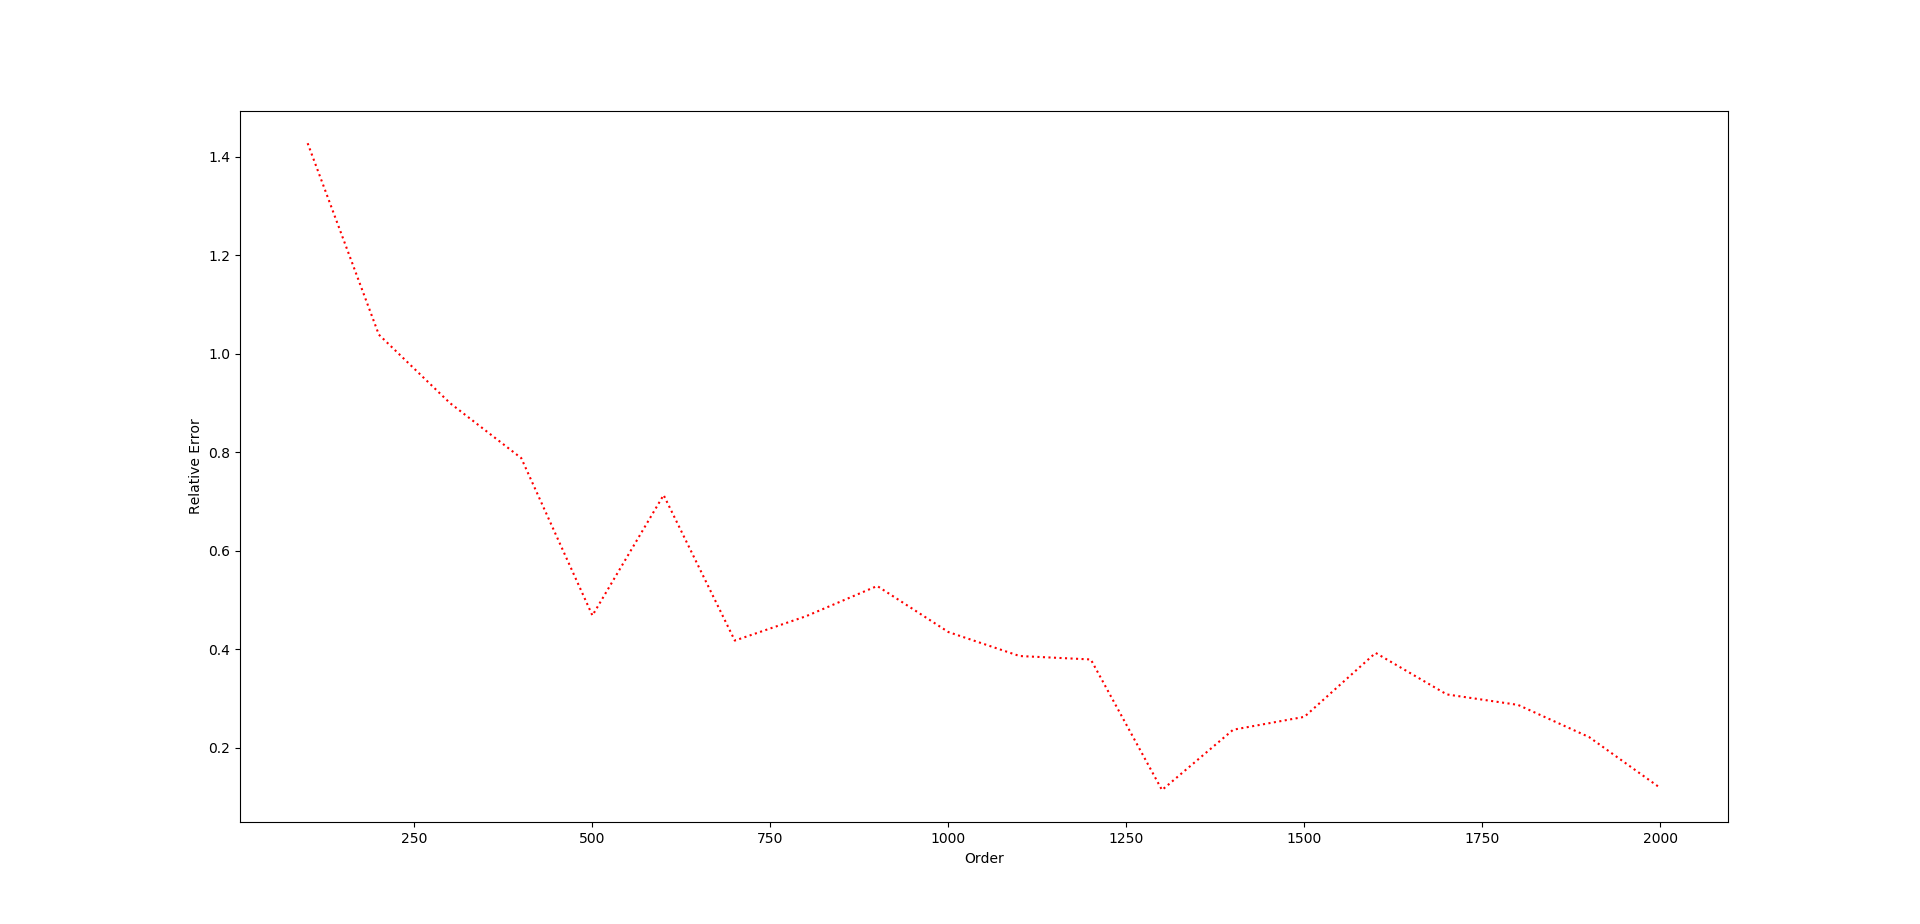
\includegraphics[width=0.75\textwidth]{ran_log_det}
	\end{center}
	\caption{The Relative Error in Several Orders of $m$}
	\label{fig9}
\end{figure}
It is clear that with the increase of $m$, relative error will be smaller. However, the computional process will also be more expensive. Therefore, we need to find a compromise to balance accuracy and speed. Form the above figure, when $m$ is larger than 1000, there is no significant promotion for the accuracy, so we may choose this value as the candidate.\\
To quantitively illustrate the improvement of accuracy with the increasing of $m$, we choose a set of $m$ and test ten times on a same $100\times 100$ matrix to calculate the relative error.
\begin{table}[htbp]
	\centering
	\caption{Absolute Error for Randomized Algorithm}
	\begin{tabular}{cccccccc}
		\toprule
		\multicolumn{1}{p{11.165em}}{\diagbox{Test Number}{Order}} & 100   & 300   & 500   & 700   & 1000  & 1500  & 2000 \\
		\midrule
		1     & 145.597 & 96.700 & 77.034 & 72.089 & 37.089 & 19.842 & 10.905 \\
		2     & 131.597 & 86.498 & 70.556 & 45.041 & 45.937 & 32.231 & 10.382 \\
		3     & 133.044 & 80.895 & 63.682 & 59.687 & 56.508 & 44.815 & 22.567 \\
		4     & 148.065 & 88.903 & 68.256 & 54.253 & 46.606 & 33.112 & 9.529 \\
		5     & 142.753 & 94.245 & 86.532 & 58.461 & 44.789 & 28.754 & 10.332 \\
		6     & 142.147 & 88.578 & 64.658 & 44.659 & 28.135 & 35.047 & 25.007 \\
		7     & 130.977 & 81.576 & 84.117 & 58.153 & 27.708 & 31.137 & 34.721 \\
		8     & 138.851 & 80.015 & 55.620 & 56.821 & 42.120 & 30.358 & 11.591 \\
		9     & 145.130 & 90.910 & 74.832 & 49.735 & 44.165 & 11.875 & 36.380 \\
		10    & 136.260 & 80.250 & 64.140 & 66.442 & 44.883 & 42.294 & 15.118 \\
		\bottomrule
	\end{tabular}%
	\label{tab2}%
\end{table}%
From Table \ref{tab2}, Randomized Algorithm is indeed improved significantly with the increase of $m$.


\subsubsection{Performance Evaluation of Parallel Acceleration}
In order to show the effectiveness of parallel acceleration on Gaussian Process, we compare the iteration time during trainging betwwen accelerated version with unaccelerated version. The result is as following:
\begin{figure}[H]
	\centering
	\subfigure[Unaccelerated]{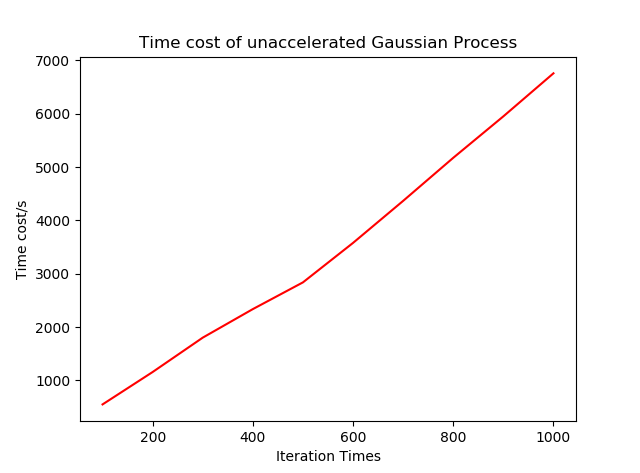
\includegraphics[width=2.7in]{time_unGP}}
	\subfigure[Accelerated]{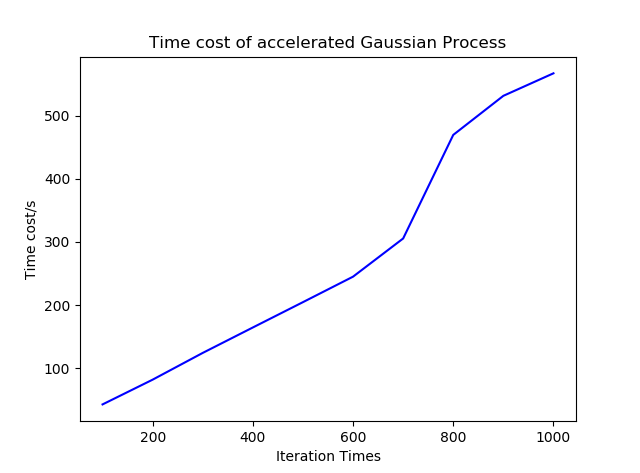
\includegraphics[width=2.7in]{time_GP}}
	\caption{Comparison of Two Implementations in Time Cost}
	\label{fig10}
\end{figure}
From the comparison, we can see the accelerated version is about 10 times faster than the unaccelerated version, this mean that we have successfully improve the scalability of Gaussian Process over large datasets.


\section{Discussion}
In this paper, we discuss the implementation details for Gaussian Process and associated accelerated techniques. There are still some questions that need more discussion.
\paragraph{Parallel potential of randomized algorithm} During the comparison of the time cost between the unaccelerated and accelerated GP, we set $m$ to be a relatively small number, however, this could have some negative influence on the accuracy. Due to the fully parallel property of this algorithm with no dependent during each iteration, this algorithm can be actually accelerated to a much larger extent (each iteration is calculated by a sub-process) as long as we have enough computational resourses. Therefore, we can improve the speed significantly while ensuring the same accuracy.
\paragraph{Parameter initialization of Adam optimizer} During the traing of Gaussian Process, the parameter initialization has a great influence on the convergence speed. Through the tests, when the parameters are well-initialized, it only takes less than 1000 iterations before the algorithm converges; when the parameters are ill-initialized, it may takes thousands of iterations. Therefore, a efficient parameter initialization strategy should be implemented to takcle the trainging of GP. Also, there is another interesting discovery to mention. That is , when the parameters are randomly initialized among positive and negative numbers, the final training result may appear in a pair of opposite numbers, this is due to the reason that loss function is the even function.
\paragraph{Loss of orthogonality in Lanczos tridiagonalization} The reason why the loss of orthogonality could lead to an inaccurate estimate of $log|K|$ can also be further investigated. Through the experiment, I find that when the loss of orthogonality happens in the iterations, it will produce a bunch of copies of the existed eigen value for $T$, and we know the determinant can be calculated by $|T|=\prod_{i=1}^{n}\lambda_i$, as the eigen values of $T$ no longer equal to that of $K$, it is clear that their determinant are not equal.

\paragraph{Blackbox framework for Gaussian process interence} A blackbox framework which only needs the users provide the datasets needs further investigations. Although Gpytorch paper already presents a blackbox framework, but it still suffers from the problems of numerical stability. In this paper, I have not figured out a way to combine the CG algorithm with Randomized Algorithm. However, through referring to some literatures, there is possibility of combining partial Lanczos Tridiagonalization with CG algorithm.

\paragraph{Multi-output Gaussian process} I think a parallel computational approach targeted at multi-output Gaussian process is  a possible research topic in the future. In this paper, I have dealed with multi-input features by norm operation, however, it still could not produce multi-output features. Recently, the multi-output property is essential as multi-output classifier is the most common and basic one in machine learning. There are already some papers to takcle the multi-output Gaussian Process. For example, B. Wang proposed a Gaussian process regression with multiple response variables \cite{16}, E.V. Bonilla proposed a multi-task Gaussian process prediction \cite{17}. But neither of them use some acceleration techniques to improve the scalability of the Gaussian Process. In view of the necessity of multi-output models, this will be a competitive research topic.

\newpage
\bibliographystyle{unsrt}  
%\bibliography{references}  %%% Remove comment to use the external .bib file (using bibtex).
%%% and comment out the ``thebibliography'' section.


%%% Comment out this section when you \bibliography{references} is enabled.
\begin{thebibliography}{1}

\bibitem{1}
Rasmussen, Carl Edward. "Gaussian processes in machine learning." Summer School on Machine Learning. Springer, Berlin, Heidelberg, 2003.

\bibitem{2}
Girard, Agathe, et al. "Gaussian process priors with uncertain inputs application to multiple-step ahead time series forecasting." Advances in neural information processing systems. 2003.

\bibitem{3}
Wilson, Andrew Gordon. Covariance kernels for fast automatic pattern discovery and extrapolation with Gaussian processes. Diss. University of Cambridge, 2014.

\bibitem{4}
Datta, Biswa Nath. Numerical linear algebra and applications. Vol. 116. Siam, 2010.

\bibitem{5}
J. W. Demmel. Applied numerical linear algebra, volume 56. Siam, 1997. 

\bibitem{6}
Bach, Francis. "Sharp analysis of low-rank kernel matrix approximations." Conference on Learning Theory. 2013.

\bibitem{7}
Fitzsimons, Jack K., et al. "Improved stochastic trace estimation using mutually unbiased bases." arXiv preprint arXiv:1608.00117 (2016).

\bibitem{8}
Kingma, Diederik P., and Jimmy Ba. "Adam: A method for stochastic optimization." arXiv preprint arXiv:1412.6980 (2014).

\bibitem{9}
P. Cortez and A. Morais. A Data Mining Approach to Predict Forest Fires using Meteorological Data. In J. Neves, M. F. Santos and J. Machado Eds., New Trends in Artificial Intelligence, Proceedings of the 13th EPIA 2007 - Portuguese Conference on Artificial Intelligence, December, Guimarães, Portugal, pp. 512-523, 2007. APPIA, ISBN-13 978-989-95618-0-9.

\bibitem{10}
Kelley, Carl T. Iterative methods for optimization. Society for Industrial and Applied Mathematics, 1999.

\bibitem{11}
Harbrecht, Helmut, Michael Peters, and Reinhold Schneider. "On the low-rank approximation by the pivoted Cholesky decomposition." Applied numerical mathematics 62.4 (2012): 428-440.

\bibitem{12}
Fika, Paraskevi, and Christos Koukouvinos. "Stochastic estimates for the trace of functions of matrices via Hadamard matrices." Communications in Statistics-Simulation and Computation 46.5 (2017): 3491-3503.

\bibitem{13}
Lanczos, Cornelius. An iteration method for the solution of the eigenvalue problem of linear differential and integral operators. Los Angeles, CA: United States Governm. Press Office, 1950.

\bibitem{14}
Boutsidis, Christos, et al. "A randomized algorithm for approximating the log determinant of a symmetric positive definite matrix." Linear Algebra and its Applications 533 (2017): 95-117.

\bibitem{15}
Simon, Horst D. "The Lanczos algorithm with partial reorthogonalization." Mathematics of computation 42.165 (1984): 115-142.

\bibitem{16}
Wang, Bo, and Tao Chen. "Gaussian process regression with multiple response variables." Chemometrics and Intelligent Laboratory Systems 142 (2015): 159-165.

\bibitem{17}
Bonilla, Edwin V., Kian M. Chai, and Christopher Williams. "Multi-task Gaussian process prediction." Advances in neural information processing systems. 2008.
\end{thebibliography}
\end{document}
